% vim: set spl=en:
\documentclass[smaller,t]{beamer}
\usepackage[utf8]{inputenc}
\usetheme{westlife}

\def\code#1{\structure{\texttt{#1}}}
\def\nadpis#1{\par\medskip\textbf{#1}}

\begin{document}
\makeatletter

\title{Virtualized Web Portals in EGI \\[\smallskipamount] Federated Cloud}
\date{ISGC 2017, Taipei, March 5--10}
\author[A. Křenek et al.]{Aleš Křenek et al.}
\begin{frame}
\maketitle
\end{frame}

\begin{frame}{Web portals in the cloud}

\textbf{Web portal advantages}
\begin{itemize}
\item The user is scientist, not IT enthusiast
\item Shield him/her from complexity of application and infrastructure
\item Easy use, reproducible results
\end{itemize}

\pause
\textbf{Drawbacks}
\begin{itemize}
\item Application and infra are complex, the portal is twice more
\item Hand-crafted, ``don't touch and run for ever''
\end{itemize}

\pause
\textbf{Go to cloud}
\begin{itemize}
\item Reproducible, automated deployment
\item More flexible and scalable setup
\end{itemize}

% machine readable documentation

\end{frame}

\begin{frame}{(How) it works}

\centering
This is a very nice schema with several \alert{important highlights.}

% \leavevmode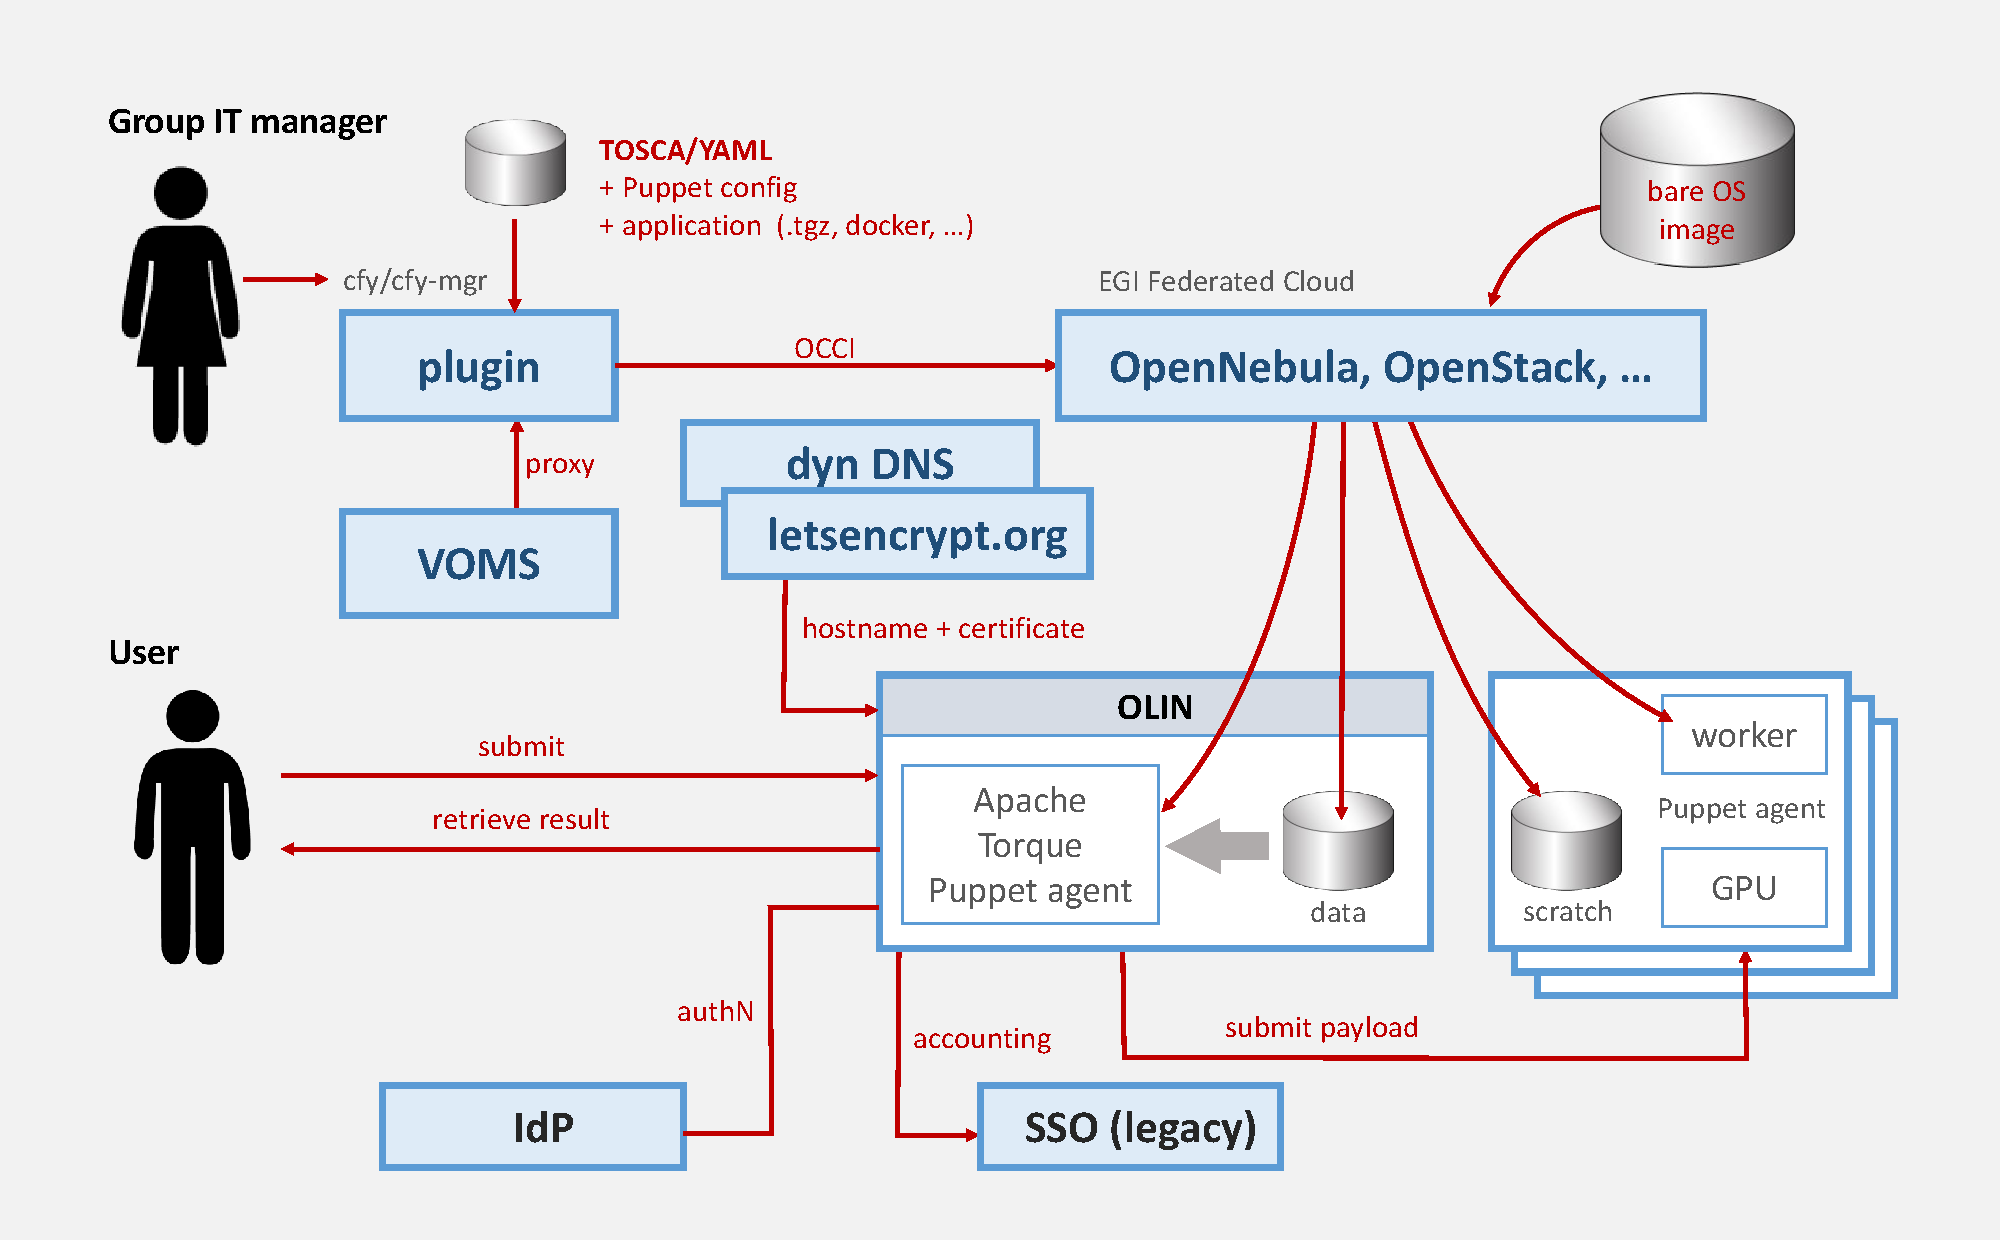
\includegraphics[height=.6\paperheight]{schema_export.pdf}


\end{frame}

\end{document}
